\chapter{The Standard Model}
\label{chap:I-1-standard-model}

  The standard model provides a classification and description of the subatomic particles that compose our universe and their interactions. It describes both the particles of matter called fermions, which are subdivied among quarks and leptons, and the force carriers named bosons. Figure \ref{fig:I-1-sm-particles} gives a schematic view of the particle content of the standard model and the ways they are classified. Quarks and leptons are further divided into three generations, with identical properties but increasing mass, from which the first constitutes the everyday matter while the two others quickly decay towards lower generations. The interaction of fermions with each other is carried out through the exchange of bosons. Gluons are the carriers of the strong force and interract solely with themselves and quarks as described by QCD. The photon, responsable for electromagnetism couples to all charged particles while the $ W^\pm $ and $ Z $ bosons couple to all particles except gluons as described by EWK. Finally, the Higgs boson as previously stated is the manifestation of the Higgs mechanism at the origin of mass. \\

	\begin{figure}[h!]
		\centering
		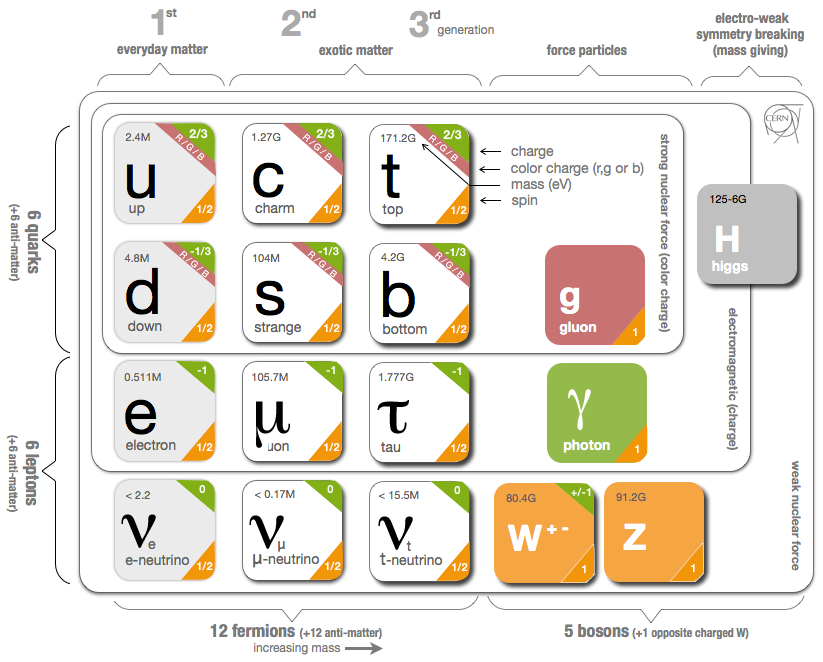
\includegraphics[width = 0.8 \textwidth]{img/I-1/sm-particles.png}
		\caption{Overview of the elementary particles as described by the standard model. Everyday matter is composed of the first generation of quarks and leptons to which two generations of heavier declinaisions are added. Gauge bosons or force particles are the carriers of the interactions between other particles. The Higgs boson is the manifestation of the mechanism that gives mass to particles [CERN].}
		\label{fig:I-1-sm-particles}
	\end{figure}

  Besides classifying particles, the standard model also provide as strong mathematical model built on top of quantum field theory and gauge invariance. The gauge group of the theory is $ SU(3)_C \otimes SU(2)_L \otimes U(1)_Y $, where $ SU(3)_C $ and $ SU(2)_L \otimes U(1)_Y $ are respectivly the symetry groups of the QCD and EWK sectors. Quarks and leptons are represented as fermionic fields within the Lagrangian of the model while bosons arise from the invariance of the Lagrangian under local gauge transformations. \\

  \section{Gauge Invariance and Gauge Bosons}

    A local transformation of a fermionic field $ \psi $ under a gauge group $ G $  can be written as
    \begin{equation}
      \psi \rightarrow \psi' = \exp\left(- \frac{i}{2} g \alpha^k(x) T^k \right) \psi ,
    \end{equation}
    where $ g $ is the gauge coupling constante, $ \alpha^k(x) $ are the local rotation paramters, and $ T^k $ are the generators of the representation of $ G $. To preserve the invariance of the Lagrangian of a free massless field $ \psi $,
    \begin{equation}
      \mathcal{L} = i \bar{\psi} \gamma^\mu \partial_\mu \psi ,
    \end{equation}
    the partial derivate $ \partial_\mu $ must be rewriten as a covariant derivate
    \begin{equation}
      D_\mu = \partial_\mu - \frac{i g}{2} W^k_\mu T^k ,
    \end{equation}
    where $ W^k_\mu $ are the emerging gauge fields associated to $ G $. The gauge invaratiant Lagrangian thus becomes
    \begin{equation}
      \mathcal{L} = i \bar{\psi} \gamma^\mu D_\mu \psi - \frac{1}{4} W^i_{\mu \nu} W^{i \mu \nu} ,
    \end{equation}
    where $ W^i_{\mu \nu} $ are the field strength tensors of the $ W^i_\mu $ gauge fields given by
    \begin{equation}
      W^i_{\mu \nu} = \partial_\mu W^i_\nu - \partial_\nu W^i_\mu - g \epsilon^{ijk} W^j_\nu W^k_\mu ,
    \end{equation}
    with $ \epsilon^{ijk} $ the totaly antisymetrical tensor. Interaction terms between the fermionic field $ \psi $ and the gauge fields $ W^i_\mu $ as well as self-interacting gauge field terms have emerged from the necessity of the invariance of the theory under local transformations. A new massless gauge boson is associated to each generator of the adjoint representation of the symetry group $ G $.

  \section{Electroweak Theory}

    The gauge group of the EWK sector of the standard model is $ SU(2)_L \otimes U(1)_Y $ for which a transformation of a field $ \psi $ can be written as
    \begin{equation}
      \psi \rightarrow \psi' = \exp\left(- \frac{i}{2} g_W \Lambda^k(x) T^k \right) \exp\left(- \frac{i}{2} g_W' \alpha(x) Y \right) \psi ,
    \end{equation}
    where $ g_W $, $ \Lambda^k(x) $, and $ T^k $ are respectivly the gauge coupling, local rotation parameters, and represenation of the $ SU(2)_L $ weak isospin algebra and $ g_W' $, $ \alpha(x) $, and $ Y $ are their $ U(1)_Y $ hypercharge algebra counterparts. The corresponding covariant derivate is
    \begin{equation}
      D_\mu = \partial_\mu - \frac{i g_W}{2} W^k_\mu T^k - \frac{i g_W'}{2} B_\mu Y ,
    \end{equation}
    where $ W^k_\mu $ and $ B_\mu$ are the emerging gauge fields associated to $ SU(2)_L $ and $ U(1)_Y $. \\

    Each fermion can couple differently to the gauge fields according to the representation of the $ SU(2)_L $ group they are part of. To determine the coupling constants it is important to separate each fermionic field into its left-handed and right-handed components such that
    \begin{equation}
      \psi = \psi_L + \psi_R \equiv \gamma^L \psi + \gamma^R \psi ,
    \end{equation}
    with
    \begin{align}
      \gamma^{L/R} & = \frac{1}{2} \left( 1 \mp \gamma^5 \right) \ \text{and} \\
      \gamma^5 & = i \gamma^0 \gamma^1 \gamma^2 \gamma^3 ,
    \end{align}
    where $ \gamma^\mu $ are the Dirac matrices. It has been showed experimentatly that only left-handed particles interact with the $ SU(2)_L $ group, meaning that right-handed particles are part of the trivial representation of the group while left-handed particles are part of the fundamental representation which generators are given by Pauli's matrices. Particles are thus grouped as follows:
    \begin{itemize}
      \item leptons: $ e_R $, $ \mu_R $, $ \tau_R $, $ \left( \begin{matrix} \nu_e \\ e \end{matrix} \right)_L $, $ \left( \begin{matrix} \nu_\mu \\ \mu \end{matrix} \right)_L $, and $ \left( \begin{matrix} \nu_\tau \\ \tau \end{matrix} \right)_L $ ;
      \item quarks: $ u_R $, $ d_R $, $ c_R $, $ s_R $, $ t_R $, $ b_R $, $ \left( \begin{matrix} u \\ d \end{matrix} \right)_L $, $ \left( \begin{matrix} c \\ s \end{matrix} \right)_L $, and $ \left( \begin{matrix} t \\ b \end{matrix} \right)_L $.
    \end{itemize}
    Note that the right-handed neutrinos are not present as they do not interact with particles and are thus sterile. \\

    To each particle, a weak isospin $ T_3 $ can be associated, corresponding to the Casimir operator of $ SU(2)_L $. Right-handed particles have $ T_3 = 0 $, positive quarks and neutrinos have $ T_3 = \frac{1}{2} $, and negative quarks and charged leptons have $ T_3 = - \frac{1}{2} $. The same can be done for the $ U(1)_Y $ group for which an hypercharge $ Y $ is defined. Through breaking of the symetry as explained in the next section, a new relation can be obtained:
    \begin{equation}
      Q = T_3 + Y ,
    \end{equation}
    where $ Q $ is the electric charge of the particle.

  \section{Electroweak Symetry Breaking}

    The physical fields of the photon $ A_\mu $ and the weak interaction bosons $ W^\pm_\mu $ and $ Z_\mu $ are linear combination of the $ B_\mu $ and $ W^i_\mu $ gauge fields. This is a consequence of the higgs mechanism that gives masses to the $ W^\pm $ and $ Z $ bosons but leaves the photon massless, thus breaking the gauge symetry of EWK under $ SU(2)_L \otimes U(1)_Y $ into a $ U(1)_{em} $ symetry group. \\

    To account for the masses of particles, R. Brout, F. Englert, and P. W. Higgs postulated the existance of a scalar doublet in $ SU(2)_L $ with hypercharge $ Y = \frac{1}{2} $
    \begin{equation}
      \phi = \left( \begin{matrix} \phi^+ \\ \phi^0 \end{matrix} \right)
    \end{equation}
    for which the Lagrangian can be written as
    \begin{equation}
      \mathcal{L} = \left( D_\mu \phi \right)^\dagger \left( D^\mu \phi \right) - V(\phi^\dagger \phi)
    \end{equation}
    with $ D_\mu $ the covariant derivate of the $ SU(2)_L \otimes U(1)_Y $ gauge groupe, and $ V $ the potential of the so called Higgs field. The chosen form of $ V $,
    \begin{equation}
      V(\phi^\dagger \phi) = \lambda \left( \phi^\dagger \phi \right)^2 - \mu^2 \phi^\dagger \phi ,
    \end{equation}
    is where the symetry breaking occurs as the ground state of the system is reached when
    \begin{equation}
      \left| \phi \right| = \sqrt{\frac{\mu^2}{2 \lambda}} = \frac{v}{\sqrt{2}} .
    \end{equation}
    The spountaneous breakdown of the symetry accounts for the creation of three Nambu-Goldstone bosons which give their masses to the three weak interaction bosons, and one new field $ H $, the Higgs field. It can be shown that the masses of these particles are directly proportionnal to $ v $:
    \begin{align}
      m_H & = \sqrt{2 \lambda} v \\
      m_Z & = \frac{1}{2} \sqrt{g_W^2 + g_W^2\text{'}} \\
      m_W & = \frac{1}{2} v g .
    \end{align}
    Giving masses to fermionic fields occurs through coupling to the $ \phi $ doublet which respects the gauge invariance of $ SU(2)_L \otimes U(1)_Y $
    \begin{equation}
      \mathcal{L} = - \lambda \bar{\psi}_L \phi \psi_R + h.c.
    \end{equation} \\

    Requiring that the photon field $ A_\mu $ be massless, a linear combination of the $ B_\mu $ and $ W^i_\mu $ must be done
    \begin{align}
      A_\mu & = W^3_\mu \sin \theta_W + B_\mu \cos \theta_W , \\
      Z_\mu & = W^3_\mu \cos \theta_W - B_\mu \sin \theta_W , \\
      W^\pm_\mu & = \frac{1}{\sqrt{2}} \left( W^1_\mu \mp i W^2_\mu \right) \text{and}
    \end{align}
    with
    \begin{equation}
      \tan \theta_W = \frac{g_W'}{g_W} ,
    \end{equation}
    where $ \theta_W $ is the weak mixing or Weinberg angle. From this transformation, it is easy to compute the coupling strengths of particles to the photon field and more particularly the coupling of the positron to the photon
    \begin{equation}
      e = g_w \sin \theta_W .
    \end{equation}

  \section{Quantum Chromodynamics}

    QCD uses the $ SU(3)_C $ gauge group to describe the behaviour of quarks and gluons, and introduces the notion of colour charge. After the observation of particles composed of three identical quarks in the same spin configuration, a new quantum number had to be introduced in order to obey Pauli's exclusion principle. Through their symetry under the $ SU(3)_C $ group, quarks carry a colour (red, blue, or green) that is changed by the interaction with gluons. However, as given quark configurations are not observed experimentaly, a constraint was added and forced hadrons (quark groupments) to be colorless: compoused of a quark and an antiquark of opposite color, or composed of three quarks of different color. \\

    Quarks are placed in the fundamental representation of the $ SU(3)_C $ group which are triplets of the same quark with the three different colours while leptons are singlets as they do not interact under QCD. The convariant derivate becomes
    \begin{equation}
      D_\mu = \partial_\mu - \frac{i g_S}{2} G^a_\mu \lambda^a
    \end{equation}
    where $ g_S $ is the strong coupling constant, $ G^a $ are the 8 gluon gauge fields, and $ \lambda^a $ are the Gell-Mann matrices. Gluons are massless as they do not interact with the Higgs fields.

  \section{Beyond the Standard Model}

    Although the standard model provides a very accurate description of the QCD and EWK theories it bares some shortcomings in order to be considered to be the theory of everything. \\

    QCD and EWK theories have been combined in the standard model to account for strong, weak, and electromagnetic forces, but including Einstein's theory of general relativity, which describes gravitationnal forces, still remains a challenge. Some theories propose to add a particle to the model, the graviton, but fail to describe all phenomena experimentally observed. To this day, general relativity remains the prominent theory of gravitation, validated by the recent discovery of gravitaionnal waves by the LIGO experiment in February 2016 \cite{PhysRevLett.116.061102}. \\

    The success of the unification of the weak and electromagnetic forces into a single EWK theory has motivated physicists to unify QCD and EWK into a single force at high energies. This implies a symetry breaking mechanism similar to the Higgs mechanism at low energies and thus the existence of new particles undetected as of today. \\

    Although general relativity provides predictions that have been experimentaly tested with great precision, it fails to account for effects such as the excessive rotation speed of galaxies or gravitanionnal lensing. Instead of rewritting Einstein's theory, the existence of dark matter and energy has been postulated which would interact gravitationnaly but not by any other force. From computation, only 5\% of our universe would be composed of standard model particles while the remaining 95\% is made of yet unknown matter and energy. \\

    Furthermore, the standard model as it is written fails to give mass to the neutrinos while experimental results have proven that neutrinos, although very light, carry a mass. Moreover, neutrino oscillations between generations have been observed by Super-Kamiokande in 1998 \cite{Fukuda:1998mi}, meaning that the standard model neutrinos are not the mass eigen states. \\

    These examples are only a few of the questions that remain open. To answer some of them, physicists need to reach higher energies in order to explore new sectors of physics unaccessible under normal conditions. To reach that goal, powerfull machines such as particle colliders have been build. The latest achivement in this field is the construction of the LHC at CERN.
